\documentclass[twoside]{book}

% Packages required by doxygen
\usepackage{fixltx2e}
\usepackage{calc}
\usepackage{doxygen}
\usepackage[export]{adjustbox} % also loads graphicx
\usepackage{graphicx}
\usepackage[utf8]{inputenc}
\usepackage{makeidx}
\usepackage{multicol}
\usepackage{multirow}
\PassOptionsToPackage{warn}{textcomp}
\usepackage{textcomp}
\usepackage[nointegrals]{wasysym}
\usepackage[table]{xcolor}

% Font selection
\usepackage[T1]{fontenc}
\usepackage[scaled=.90]{helvet}
\usepackage{courier}
\usepackage{amssymb}
\usepackage{sectsty}
\renewcommand{\familydefault}{\sfdefault}
\allsectionsfont{%
  \fontseries{bc}\selectfont%
  \color{darkgray}%
}
\renewcommand{\DoxyLabelFont}{%
  \fontseries{bc}\selectfont%
  \color{darkgray}%
}
\newcommand{\+}{\discretionary{\mbox{\scriptsize$\hookleftarrow$}}{}{}}

% Page & text layout
\usepackage{geometry}
\geometry{%
  a4paper,%
  top=2.5cm,%
  bottom=2.5cm,%
  left=2.5cm,%
  right=2.5cm%
}
\tolerance=750
\hfuzz=15pt
\hbadness=750
\setlength{\emergencystretch}{15pt}
\setlength{\parindent}{0cm}
\setlength{\parskip}{0.2cm}
\makeatletter
\renewcommand{\paragraph}{%
  \@startsection{paragraph}{4}{0ex}{-1.0ex}{1.0ex}{%
    \normalfont\normalsize\bfseries\SS@parafont%
  }%
}
\renewcommand{\subparagraph}{%
  \@startsection{subparagraph}{5}{0ex}{-1.0ex}{1.0ex}{%
    \normalfont\normalsize\bfseries\SS@subparafont%
  }%
}
\makeatother

% Headers & footers
\usepackage{fancyhdr}
\pagestyle{fancyplain}
\fancyhead[LE]{\fancyplain{}{\bfseries\thepage}}
\fancyhead[CE]{\fancyplain{}{}}
\fancyhead[RE]{\fancyplain{}{\bfseries\leftmark}}
\fancyhead[LO]{\fancyplain{}{\bfseries\rightmark}}
\fancyhead[CO]{\fancyplain{}{}}
\fancyhead[RO]{\fancyplain{}{\bfseries\thepage}}
\fancyfoot[LE]{\fancyplain{}{}}
\fancyfoot[CE]{\fancyplain{}{}}
\fancyfoot[RE]{\fancyplain{}{\bfseries\scriptsize Generated on Mon Dec 14 2015 23\+:56\+:52 for Project 2 by Doxygen }}
\fancyfoot[LO]{\fancyplain{}{\bfseries\scriptsize Generated on Mon Dec 14 2015 23\+:56\+:52 for Project 2 by Doxygen }}
\fancyfoot[CO]{\fancyplain{}{}}
\fancyfoot[RO]{\fancyplain{}{}}
\renewcommand{\footrulewidth}{0.4pt}
\renewcommand{\chaptermark}[1]{%
  \markboth{#1}{}%
}
\renewcommand{\sectionmark}[1]{%
  \markright{\thesection\ #1}%
}

% Indices & bibliography
\usepackage{natbib}
\usepackage[titles]{tocloft}
\setcounter{tocdepth}{3}
\setcounter{secnumdepth}{5}
\makeindex

% Hyperlinks (required, but should be loaded last)
\usepackage{ifpdf}
\ifpdf
  \usepackage[pdftex,pagebackref=true]{hyperref}
\else
  \usepackage[ps2pdf,pagebackref=true]{hyperref}
\fi
\hypersetup{%
  colorlinks=true,%
  linkcolor=blue,%
  citecolor=blue,%
  unicode%
}

% Custom commands
\newcommand{\clearemptydoublepage}{%
  \newpage{\pagestyle{empty}\cleardoublepage}%
}


%===== C O N T E N T S =====

\begin{document}

% Titlepage & ToC
\hypersetup{pageanchor=false,
             bookmarks=true,
             bookmarksnumbered=true,
             pdfencoding=unicode
            }
\pagenumbering{roman}
\begin{titlepage}
\vspace*{7cm}
\begin{center}%
{\Large Project 2 }\\
\vspace*{1cm}
{\large Generated by Doxygen 1.8.10}\\
\vspace*{0.5cm}
{\small Mon Dec 14 2015 23:56:52}\\
\end{center}
\end{titlepage}
\clearemptydoublepage
\tableofcontents
\clearemptydoublepage
\pagenumbering{arabic}
\hypersetup{pageanchor=true}

%--- Begin generated contents ---
\chapter{Hierarchical Index}
\section{Class Hierarchy}
This inheritance list is sorted roughly, but not completely, alphabetically\+:\begin{DoxyCompactList}
\item \contentsline{section}{Is\+Valid}{\pageref{class_is_valid}}{}
\begin{DoxyCompactList}
\item \contentsline{section}{Game$<$ T $>$}{\pageref{class_game}}{}
\end{DoxyCompactList}
\end{DoxyCompactList}

\chapter{Class Index}
\section{Class List}
Here are the classes, structs, unions and interfaces with brief descriptions\+:\begin{DoxyCompactList}
\item\contentsline{section}{\hyperlink{class_game}{Game$<$ T $>$} }{\pageref{class_game}}{}
\item\contentsline{section}{\hyperlink{class_is_valid}{Is\+Valid} }{\pageref{class_is_valid}}{}
\end{DoxyCompactList}

\chapter{File Index}
\section{File List}
Here is a list of all files with brief descriptions\+:\begin{DoxyCompactList}
\item\contentsline{section}{Project\+\_\+v5/\hyperlink{_8dep_8inc}{.\+dep.\+inc} }{\pageref{_8dep_8inc}}{}
\item\contentsline{section}{Project\+\_\+v5/\hyperlink{_game_8cpp}{Game.\+cpp} }{\pageref{_game_8cpp}}{}
\item\contentsline{section}{Project\+\_\+v5/\hyperlink{_game_8h}{Game.\+h} }{\pageref{_game_8h}}{}
\item\contentsline{section}{Project\+\_\+v5/\hyperlink{_is_valid_8cpp}{Is\+Valid.\+cpp} }{\pageref{_is_valid_8cpp}}{}
\item\contentsline{section}{Project\+\_\+v5/\hyperlink{_is_valid_8h}{Is\+Valid.\+h} }{\pageref{_is_valid_8h}}{}
\item\contentsline{section}{Project\+\_\+v5/\hyperlink{_main_8cpp}{Main.\+cpp} }{\pageref{_main_8cpp}}{}
\item\contentsline{section}{Project\+\_\+v5/build/\+Debug/\+Cygwin\+\_\+4.\+x-\/\+Windows/\hyperlink{_game_8o_8d}{Game.\+o.\+d} }{\pageref{_game_8o_8d}}{}
\item\contentsline{section}{Project\+\_\+v5/build/\+Debug/\+Cygwin\+\_\+4.\+x-\/\+Windows/\hyperlink{_is_valid_8o_8d}{Is\+Valid.\+o.\+d} }{\pageref{_is_valid_8o_8d}}{}
\item\contentsline{section}{Project\+\_\+v5/build/\+Debug/\+Cygwin\+\_\+4.\+x-\/\+Windows/\hyperlink{_main_8o_8d}{Main.\+o.\+d} }{\pageref{_main_8o_8d}}{}
\end{DoxyCompactList}

\chapter{Class Documentation}
\hypertarget{class_game}{}\section{Game$<$ T $>$ Class Template Reference}
\label{class_game}\index{Game$<$ T $>$@{Game$<$ T $>$}}


{\ttfamily \#include $<$Game.\+h$>$}

Inheritance diagram for Game$<$ T $>$\+:\begin{figure}[H]
\begin{center}
\leavevmode
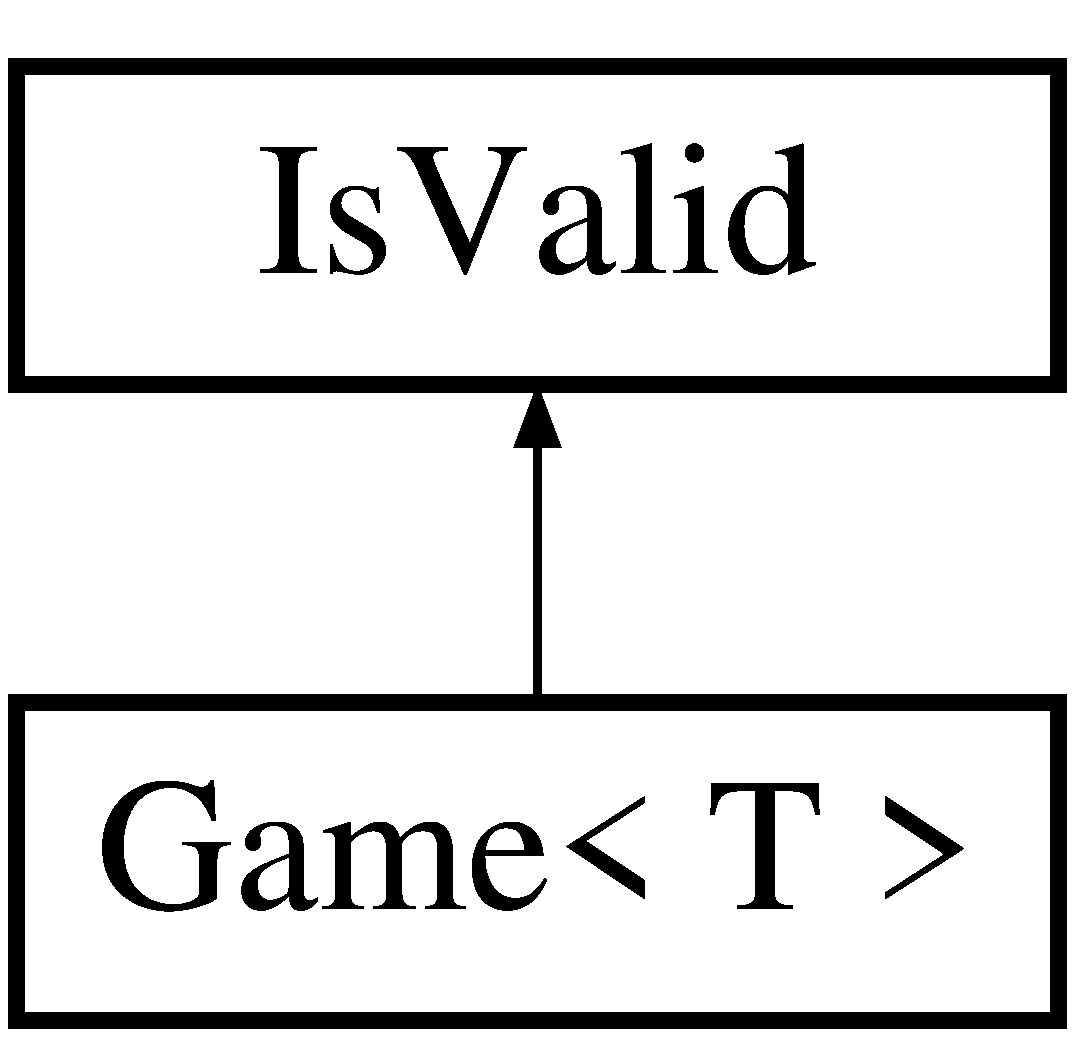
\includegraphics[height=2.000000cm]{class_game}
\end{center}
\end{figure}
\subsection*{Public Member Functions}
\begin{DoxyCompactItemize}
\item 
\hyperlink{class_game_a8d00e68144fea1d245b30021ff9a5d9b}{Game} (int level)
\item 
\hyperlink{class_game_ac98b054acf64c7ac2c7c780e79b4f618}{$\sim$\+Game} ()
\item 
short \hyperlink{class_game_acff364fb95406f49b3b0028037a787f5}{get\+Xs} () const 
\item 
short \hyperlink{class_game_a1ccc9a160aa4c0617142efbd8f654945}{get\+Os} () const 
\item 
int \hyperlink{class_game_a08ac615fa1cf399c206bcadf47109388}{get\+Guess} () const 
\item 
char $\ast$ \hyperlink{class_game_a89e9b1725d7e2e8eb3996837784e7ec4}{get\+S\+Ans} () const 
\item 
void \hyperlink{class_game_a9e6bcc1ae8e19bc25b9cfa39beb29c5a}{compare} (string \hyperlink{class_is_valid_adbf865b1f62a0967106b899e15bbc6cb}{usr\+G})
\item 
void \hyperlink{class_game_ad5e14b31647a4da393b4837d89ba57e1}{gss\+Hst} (string \hyperlink{class_is_valid_adbf865b1f62a0967106b899e15bbc6cb}{usr\+G})
\item 
void \hyperlink{class_game_ae7b3779e9ea40bceff534c31a1b4b9be}{sort} ()
\end{DoxyCompactItemize}
\subsection*{Additional Inherited Members}


\subsection{Detailed Description}
\subsubsection*{template$<$class T$>$class Game$<$ T $>$}



Definition at line 18 of file Game.\+h.



\subsection{Constructor \& Destructor Documentation}
\hypertarget{class_game_a8d00e68144fea1d245b30021ff9a5d9b}{}\index{Game@{Game}!Game@{Game}}
\index{Game@{Game}!Game@{Game}}
\subsubsection[{Game(int level)}]{\setlength{\rightskip}{0pt plus 5cm}template$<$class T $>$ {\bf Game}$<$ T $>$\+::{\bf Game} (
\begin{DoxyParamCaption}
\item[{int}]{level}
\end{DoxyParamCaption}
)}\label{class_game_a8d00e68144fea1d245b30021ff9a5d9b}


Definition at line 149 of file Game.\+h.

\hypertarget{class_game_ac98b054acf64c7ac2c7c780e79b4f618}{}\index{Game@{Game}!````~Game@{$\sim$\+Game}}
\index{````~Game@{$\sim$\+Game}!Game@{Game}}
\subsubsection[{$\sim$\+Game()}]{\setlength{\rightskip}{0pt plus 5cm}template$<$class T $>$ {\bf Game}$<$ T $>$\+::$\sim${\bf Game} (
\begin{DoxyParamCaption}
{}
\end{DoxyParamCaption}
)}\label{class_game_ac98b054acf64c7ac2c7c780e79b4f618}


Definition at line 197 of file Game.\+h.



\subsection{Member Function Documentation}
\hypertarget{class_game_a9e6bcc1ae8e19bc25b9cfa39beb29c5a}{}\index{Game@{Game}!compare@{compare}}
\index{compare@{compare}!Game@{Game}}
\subsubsection[{compare(string usr\+G)}]{\setlength{\rightskip}{0pt plus 5cm}template$<$class T$>$ void {\bf Game}$<$ T $>$\+::compare (
\begin{DoxyParamCaption}
\item[{string}]{usr\+G}
\end{DoxyParamCaption}
)\hspace{0.3cm}{\ttfamily [inline]}}\label{class_game_a9e6bcc1ae8e19bc25b9cfa39beb29c5a}


Definition at line 41 of file Game.\+h.

\hypertarget{class_game_a08ac615fa1cf399c206bcadf47109388}{}\index{Game@{Game}!get\+Guess@{get\+Guess}}
\index{get\+Guess@{get\+Guess}!Game@{Game}}
\subsubsection[{get\+Guess() const }]{\setlength{\rightskip}{0pt plus 5cm}template$<$class T $>$ int {\bf Game}$<$ T $>$\+::get\+Guess (
\begin{DoxyParamCaption}
{}
\end{DoxyParamCaption}
) const}\label{class_game_a08ac615fa1cf399c206bcadf47109388}


Definition at line 237 of file Game.\+h.

\hypertarget{class_game_a1ccc9a160aa4c0617142efbd8f654945}{}\index{Game@{Game}!get\+Os@{get\+Os}}
\index{get\+Os@{get\+Os}!Game@{Game}}
\subsubsection[{get\+Os() const }]{\setlength{\rightskip}{0pt plus 5cm}template$<$class T $>$ short {\bf Game}$<$ T $>$\+::get\+Os (
\begin{DoxyParamCaption}
{}
\end{DoxyParamCaption}
) const}\label{class_game_a1ccc9a160aa4c0617142efbd8f654945}


Definition at line 230 of file Game.\+h.

\hypertarget{class_game_a89e9b1725d7e2e8eb3996837784e7ec4}{}\index{Game@{Game}!get\+S\+Ans@{get\+S\+Ans}}
\index{get\+S\+Ans@{get\+S\+Ans}!Game@{Game}}
\subsubsection[{get\+S\+Ans() const }]{\setlength{\rightskip}{0pt plus 5cm}template$<$class T $>$ char $\ast$ {\bf Game}$<$ T $>$\+::get\+S\+Ans (
\begin{DoxyParamCaption}
{}
\end{DoxyParamCaption}
) const}\label{class_game_a89e9b1725d7e2e8eb3996837784e7ec4}


Definition at line 243 of file Game.\+h.

\hypertarget{class_game_acff364fb95406f49b3b0028037a787f5}{}\index{Game@{Game}!get\+Xs@{get\+Xs}}
\index{get\+Xs@{get\+Xs}!Game@{Game}}
\subsubsection[{get\+Xs() const }]{\setlength{\rightskip}{0pt plus 5cm}template$<$class T $>$ short {\bf Game}$<$ T $>$\+::get\+Xs (
\begin{DoxyParamCaption}
{}
\end{DoxyParamCaption}
) const}\label{class_game_acff364fb95406f49b3b0028037a787f5}


Definition at line 225 of file Game.\+h.

\hypertarget{class_game_ad5e14b31647a4da393b4837d89ba57e1}{}\index{Game@{Game}!gss\+Hst@{gss\+Hst}}
\index{gss\+Hst@{gss\+Hst}!Game@{Game}}
\subsubsection[{gss\+Hst(string usr\+G)}]{\setlength{\rightskip}{0pt plus 5cm}template$<$class T$>$ void {\bf Game}$<$ T $>$\+::gss\+Hst (
\begin{DoxyParamCaption}
\item[{string}]{usr\+G}
\end{DoxyParamCaption}
)\hspace{0.3cm}{\ttfamily [inline]}}\label{class_game_ad5e14b31647a4da393b4837d89ba57e1}


Definition at line 90 of file Game.\+h.

\hypertarget{class_game_ae7b3779e9ea40bceff534c31a1b4b9be}{}\index{Game@{Game}!sort@{sort}}
\index{sort@{sort}!Game@{Game}}
\subsubsection[{sort()}]{\setlength{\rightskip}{0pt plus 5cm}template$<$class T$>$ void {\bf Game}$<$ T $>$\+::sort (
\begin{DoxyParamCaption}
{}
\end{DoxyParamCaption}
)\hspace{0.3cm}{\ttfamily [inline]}}\label{class_game_ae7b3779e9ea40bceff534c31a1b4b9be}


Definition at line 100 of file Game.\+h.



The documentation for this class was generated from the following file\+:\begin{DoxyCompactItemize}
\item 
Project\+\_\+v5/\hyperlink{_game_8h}{Game.\+h}\end{DoxyCompactItemize}

\hypertarget{class_is_valid}{}\section{Is\+Valid Class Reference}
\label{class_is_valid}\index{Is\+Valid@{Is\+Valid}}


{\ttfamily \#include $<$Is\+Valid.\+h$>$}

Inheritance diagram for Is\+Valid\+:\begin{figure}[H]
\begin{center}
\leavevmode
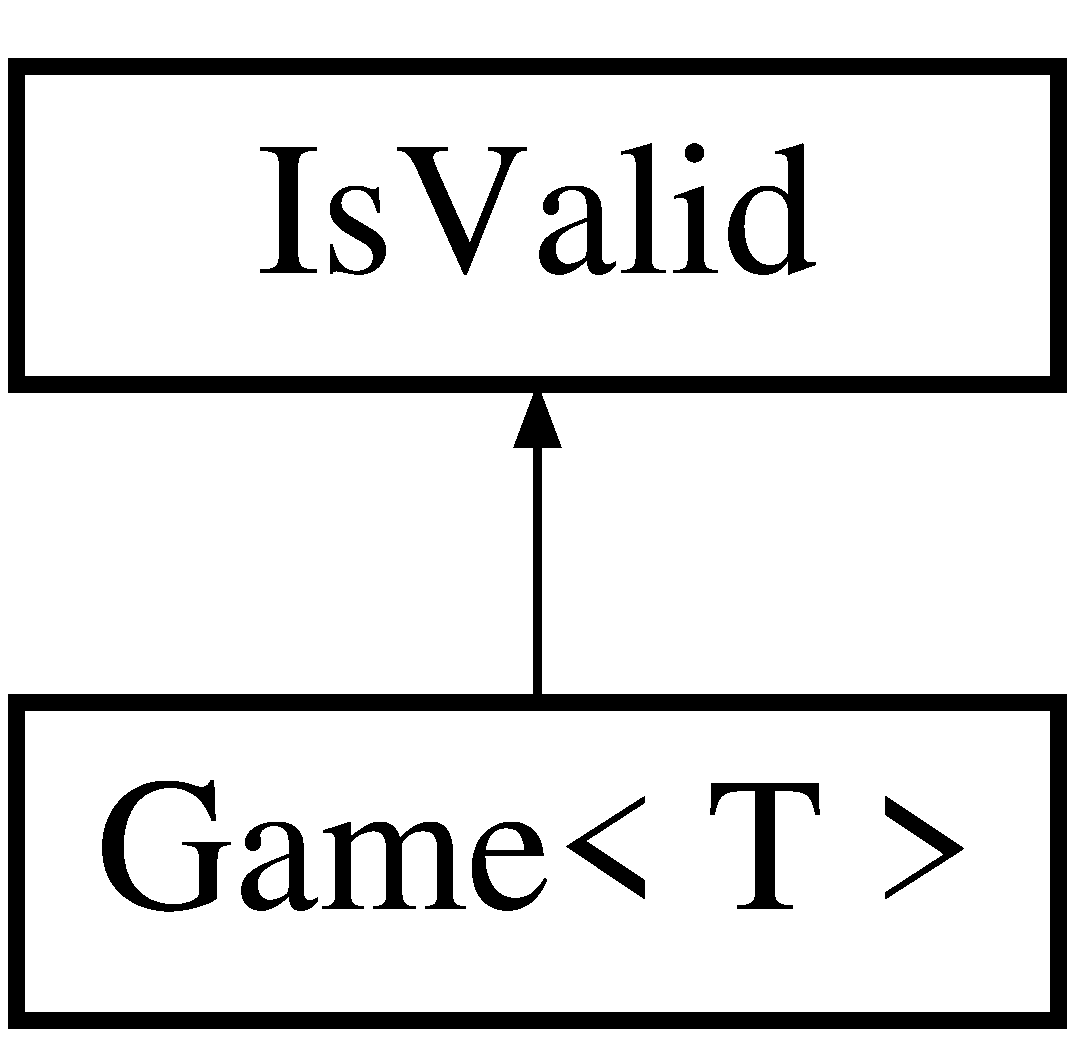
\includegraphics[height=2.000000cm]{class_is_valid}
\end{center}
\end{figure}
\subsection*{Public Member Functions}
\begin{DoxyCompactItemize}
\item 
\hyperlink{class_is_valid_ad8de07083cbd328b8643445583140ed1}{Is\+Valid} (int \hyperlink{class_is_valid_ad803e4f443a19d48af63effafc3ae527}{level})
\item 
void \hyperlink{class_is_valid_a9b09b29e31ae25d4beb6821e699c11ce}{set\+User\+G} (string \hyperlink{class_is_valid_adbf865b1f62a0967106b899e15bbc6cb}{usr\+G})
\item 
void \hyperlink{class_is_valid_ad666e24d961a3502e76769cbe4194158}{set\+Level} (int l)
\item 
bool \hyperlink{class_is_valid_aa658b1bd8bb71b55e62249047e39e938}{validate} (string)
\end{DoxyCompactItemize}
\subsection*{Protected Attributes}
\begin{DoxyCompactItemize}
\item 
string \hyperlink{class_is_valid_adbf865b1f62a0967106b899e15bbc6cb}{usr\+G}
\item 
int \hyperlink{class_is_valid_ad803e4f443a19d48af63effafc3ae527}{level}
\end{DoxyCompactItemize}


\subsection{Detailed Description}


Definition at line 16 of file Is\+Valid.\+h.



\subsection{Constructor \& Destructor Documentation}
\hypertarget{class_is_valid_ad8de07083cbd328b8643445583140ed1}{}\index{Is\+Valid@{Is\+Valid}!Is\+Valid@{Is\+Valid}}
\index{Is\+Valid@{Is\+Valid}!Is\+Valid@{Is\+Valid}}
\subsubsection[{Is\+Valid(int level)}]{\setlength{\rightskip}{0pt plus 5cm}Is\+Valid\+::\+Is\+Valid (
\begin{DoxyParamCaption}
\item[{int}]{level}
\end{DoxyParamCaption}
)\hspace{0.3cm}{\ttfamily [inline]}}\label{class_is_valid_ad8de07083cbd328b8643445583140ed1}


Definition at line 21 of file Is\+Valid.\+h.



\subsection{Member Function Documentation}
\hypertarget{class_is_valid_ad666e24d961a3502e76769cbe4194158}{}\index{Is\+Valid@{Is\+Valid}!set\+Level@{set\+Level}}
\index{set\+Level@{set\+Level}!Is\+Valid@{Is\+Valid}}
\subsubsection[{set\+Level(int l)}]{\setlength{\rightskip}{0pt plus 5cm}void Is\+Valid\+::set\+Level (
\begin{DoxyParamCaption}
\item[{int}]{l}
\end{DoxyParamCaption}
)}\label{class_is_valid_ad666e24d961a3502e76769cbe4194158}


Definition at line 17 of file Is\+Valid.\+cpp.

\hypertarget{class_is_valid_a9b09b29e31ae25d4beb6821e699c11ce}{}\index{Is\+Valid@{Is\+Valid}!set\+User\+G@{set\+User\+G}}
\index{set\+User\+G@{set\+User\+G}!Is\+Valid@{Is\+Valid}}
\subsubsection[{set\+User\+G(string usr\+G)}]{\setlength{\rightskip}{0pt plus 5cm}void Is\+Valid\+::set\+User\+G (
\begin{DoxyParamCaption}
\item[{string}]{usr\+G}
\end{DoxyParamCaption}
)}\label{class_is_valid_a9b09b29e31ae25d4beb6821e699c11ce}


Definition at line 11 of file Is\+Valid.\+cpp.

\hypertarget{class_is_valid_aa658b1bd8bb71b55e62249047e39e938}{}\index{Is\+Valid@{Is\+Valid}!validate@{validate}}
\index{validate@{validate}!Is\+Valid@{Is\+Valid}}
\subsubsection[{validate(string)}]{\setlength{\rightskip}{0pt plus 5cm}bool Is\+Valid\+::validate (
\begin{DoxyParamCaption}
\item[{string}]{a}
\end{DoxyParamCaption}
)}\label{class_is_valid_aa658b1bd8bb71b55e62249047e39e938}


Definition at line 29 of file Is\+Valid.\+cpp.



\subsection{Member Data Documentation}
\hypertarget{class_is_valid_ad803e4f443a19d48af63effafc3ae527}{}\index{Is\+Valid@{Is\+Valid}!level@{level}}
\index{level@{level}!Is\+Valid@{Is\+Valid}}
\subsubsection[{level}]{\setlength{\rightskip}{0pt plus 5cm}int Is\+Valid\+::level\hspace{0.3cm}{\ttfamily [protected]}}\label{class_is_valid_ad803e4f443a19d48af63effafc3ae527}


Definition at line 19 of file Is\+Valid.\+h.

\hypertarget{class_is_valid_adbf865b1f62a0967106b899e15bbc6cb}{}\index{Is\+Valid@{Is\+Valid}!usr\+G@{usr\+G}}
\index{usr\+G@{usr\+G}!Is\+Valid@{Is\+Valid}}
\subsubsection[{usr\+G}]{\setlength{\rightskip}{0pt plus 5cm}string Is\+Valid\+::usr\+G\hspace{0.3cm}{\ttfamily [protected]}}\label{class_is_valid_adbf865b1f62a0967106b899e15bbc6cb}


Definition at line 18 of file Is\+Valid.\+h.



The documentation for this class was generated from the following files\+:\begin{DoxyCompactItemize}
\item 
Project\+\_\+v5/\hyperlink{_is_valid_8h}{Is\+Valid.\+h}\item 
Project\+\_\+v5/\hyperlink{_is_valid_8cpp}{Is\+Valid.\+cpp}\end{DoxyCompactItemize}

\chapter{File Documentation}
\hypertarget{_8dep_8inc}{}\section{Project\+\_\+v5/.dep.\+inc File Reference}
\label{_8dep_8inc}\index{Project\+\_\+v5/.\+dep.\+inc@{Project\+\_\+v5/.\+dep.\+inc}}

\hypertarget{_game_8o_8d}{}\section{Project\+\_\+v5/build/\+Debug/\+Cygwin\+\_\+4.x-\/\+Windows/\+Game.o.\+d File Reference}
\label{_game_8o_8d}\index{Project\+\_\+v5/build/\+Debug/\+Cygwin\+\_\+4.\+x-\/\+Windows/\+Game.\+o.\+d@{Project\+\_\+v5/build/\+Debug/\+Cygwin\+\_\+4.\+x-\/\+Windows/\+Game.\+o.\+d}}

\hypertarget{_is_valid_8o_8d}{}\section{Project\+\_\+v5/build/\+Debug/\+Cygwin\+\_\+4.x-\/\+Windows/\+Is\+Valid.o.\+d File Reference}
\label{_is_valid_8o_8d}\index{Project\+\_\+v5/build/\+Debug/\+Cygwin\+\_\+4.\+x-\/\+Windows/\+Is\+Valid.\+o.\+d@{Project\+\_\+v5/build/\+Debug/\+Cygwin\+\_\+4.\+x-\/\+Windows/\+Is\+Valid.\+o.\+d}}

\hypertarget{_main_8o_8d}{}\section{Project\+\_\+v5/build/\+Debug/\+Cygwin\+\_\+4.x-\/\+Windows/\+Main.o.\+d File Reference}
\label{_main_8o_8d}\index{Project\+\_\+v5/build/\+Debug/\+Cygwin\+\_\+4.\+x-\/\+Windows/\+Main.\+o.\+d@{Project\+\_\+v5/build/\+Debug/\+Cygwin\+\_\+4.\+x-\/\+Windows/\+Main.\+o.\+d}}

\hypertarget{_game_8cpp}{}\section{Project\+\_\+v5/\+Game.cpp File Reference}
\label{_game_8cpp}\index{Project\+\_\+v5/\+Game.\+cpp@{Project\+\_\+v5/\+Game.\+cpp}}
{\ttfamily \#include \char`\"{}Game.\+h\char`\"{}}\\*

\hypertarget{_game_8h}{}\section{Project\+\_\+v5/\+Game.h File Reference}
\label{_game_8h}\index{Project\+\_\+v5/\+Game.\+h@{Project\+\_\+v5/\+Game.\+h}}
{\ttfamily \#include $<$iostream$>$}\\*
{\ttfamily \#include $<$string$>$}\\*
{\ttfamily \#include $<$cstring$>$}\\*
{\ttfamily \#include $<$ctime$>$}\\*
{\ttfamily \#include $<$cstdlib$>$}\\*
{\ttfamily \#include \char`\"{}Is\+Valid.\+h\char`\"{}}\\*
\subsection*{Classes}
\begin{DoxyCompactItemize}
\item 
class \hyperlink{class_game}{Game$<$ T $>$}
\end{DoxyCompactItemize}

\hypertarget{_is_valid_8cpp}{}\section{Project\+\_\+v5/\+Is\+Valid.cpp File Reference}
\label{_is_valid_8cpp}\index{Project\+\_\+v5/\+Is\+Valid.\+cpp@{Project\+\_\+v5/\+Is\+Valid.\+cpp}}
{\ttfamily \#include \char`\"{}Is\+Valid.\+h\char`\"{}}\\*

\hypertarget{_is_valid_8h}{}\section{Project\+\_\+v5/\+Is\+Valid.h File Reference}
\label{_is_valid_8h}\index{Project\+\_\+v5/\+Is\+Valid.\+h@{Project\+\_\+v5/\+Is\+Valid.\+h}}
{\ttfamily \#include $<$iostream$>$}\\*
{\ttfamily \#include $<$string$>$}\\*
{\ttfamily \#include $<$cstring$>$}\\*
\subsection*{Classes}
\begin{DoxyCompactItemize}
\item 
class \hyperlink{class_is_valid}{Is\+Valid}
\end{DoxyCompactItemize}

\hypertarget{_main_8cpp}{}\section{Project\+\_\+v5/\+Main.cpp File Reference}
\label{_main_8cpp}\index{Project\+\_\+v5/\+Main.\+cpp@{Project\+\_\+v5/\+Main.\+cpp}}
{\ttfamily \#include $<$iostream$>$}\\*
{\ttfamily \#include $<$string$>$}\\*
{\ttfamily \#include $<$cstdlib$>$}\\*
{\ttfamily \#include $<$fstream$>$}\\*
{\ttfamily \#include $<$ctime$>$}\\*
{\ttfamily \#include \char`\"{}Is\+Valid.\+h\char`\"{}}\\*
{\ttfamily \#include \char`\"{}Game.\+h\char`\"{}}\\*
\subsection*{Functions}
\begin{DoxyCompactItemize}
\item 
int \hyperlink{_main_8cpp_a3c04138a5bfe5d72780bb7e82a18e627}{main} (int argc, char $\ast$$\ast$argv)
\end{DoxyCompactItemize}


\subsection{Function Documentation}
\hypertarget{_main_8cpp_a3c04138a5bfe5d72780bb7e82a18e627}{}\index{Main.\+cpp@{Main.\+cpp}!main@{main}}
\index{main@{main}!Main.\+cpp@{Main.\+cpp}}
\subsubsection[{main(int argc, char $\ast$$\ast$argv)}]{\setlength{\rightskip}{0pt plus 5cm}int main (
\begin{DoxyParamCaption}
\item[{int}]{argc, }
\item[{char $\ast$$\ast$}]{argv}
\end{DoxyParamCaption}
)}\label{_main_8cpp_a3c04138a5bfe5d72780bb7e82a18e627}


Definition at line 37 of file Main.\+cpp.


%--- End generated contents ---

% Index
\backmatter
\newpage
\phantomsection
\clearemptydoublepage
\addcontentsline{toc}{chapter}{Index}
\printindex

\end{document}
